%
% Latex example file for postgrads (04/10/03)
%
% If you have questions please email me: 
% M.L.Balogh@durham.ac.uk
% or find me in room OC312.
%
% Note you can get Latex style files etc. from http://www.ctan.org


% Use emulateapj instead to make Apj format.
% YOU SHOULD REMOVE THE TABLE OF
% CONTENTS PAGE WHEN USING APJ FORMAT.
\documentclass[11pt,a4paper]{emulateapj}
\bibliographystyle{apj}


%define general packages
\usepackage{epsfig}
\usepackage{amsmath}
\usepackage{natbib}

% spanish packages
\usepackage[utf8]{inputenc}
\usepackage[spanish]{babel}
\languageshorthands{none}
\noextrasspanish
\let\layoutspanish\relax
\usepackage[spanish]{babel}
\renewcommand\shorthandsspanish{}

%internal short cuts
\def \HgA {H$\gamma_A$}
\def \gon {Gonz\'{a}lez}
\def \Hbp {H$\beta ^\prime$}
\def \warn {{\sffamily\bfseries\large WARNING, ARREGLAR:}}









\begin{document}

\submitted{Departamento Ing. en Informática, ITBA}
\title{Diseño de reactores nucleares \HgA}
\author{Aráoz M. \& Williams M.}
\date{\today}


\begin{abstract}
Entre 2 y tres oraciones.
\warn completar
ABSTRACT ABSTRACT ABSTRACT ABSTRACT ABSTRACT ABSTRACT ABSTRACT ABSTRACT ABSTRACT 
ABSTRACT ABSTRACT ABSTRACT ABSTRACT ABSTRACT ABSTRACT ABSTRACT ABSTRACT ABSTRACT 
\end{abstract}

\maketitle




\section{Introduccción}
\label{sec:introduccion}
Un reactor nuclear de fisión es un dispositivo en el que se producen reacciones nucleares
donde neutrones rompen núcleos de número atómico grande. En dicha ruptura, se
producen: 
\begin{enumerate}
	\item fragmentos de fisión, esto es núcleos con Z intermedio.
	\item neutrones que se utilizan para continuar el proceso de fusión y 
	\item energía del orden de 200MeV. Si se dan
las condiciones necesarias, este proceso es autosostenido, produciéndose una reacción en cadena.
\end{enumerate}
La energía liberada permite calentar agua que circula por un determinado circuito. Así
se genera vapor. Este vapor es utilizado para producir el movimiento de turbinas en
generadores de electricidad.

La difusión de neutrones en el núcleo de un reactor debe ser controlada, para poder mantener
la reacción en cadena. Para tal fin se utilizan medios moderadores como el agua $H_2O$
o el agua pesada $D_2O$.


En reactores autoregenerables se utiliza como combustible nuclear sales de $U^{238}_{92}$ .

Para modelar el proceso estacionario de difusión de neutrones en un reactor, consideremos
un modelo de celda de combustible y medio moderador unidimensional. La sal $UO_2$ se
encuentra en el núcleo de la celda emitiendo neutrones. Tales neutrones pasan al medio
moderador que controla la difusión. Consideremos a dicho medio agua liviana.

La ecuación de difusión nuclear para los neutrones, en estado estacionario es:
\begin{eqnarray}
\label{eq:ecuacionADiscretizar}
  -\dfrac{d}{dx}[D \dfrac{d\phi}{dx}(x)] + \sigma \phi(x)  &=& \lambda  \Sigma_f \phi(x)
\end{eqnarray}
donde $\phi$ es la concentración de neutrones, $D$ es el coeficiente de difusión neutrónica del
medio, $\sigma$ es el coeficiente de absorcion de neutrones y $\Sigma_f$ es la sección eficaz de fusión del
medio. La constante $\lambda$ depende de la geometría del reactor y por lo tanto es un parámetro
de diseño.
Para el modelo unidimensional compuesto por una celda junto a un moderador 
-cuyo diagrama se muestra en la figura \ref{fig:esquema}- las dimensiones 
lineales son $20cm$ para la celda de combustible y 10cm para la barra de moderador.
Además, en la figura, se dán los valores de $\sigma$, $D$, y $\Sigma_f$.

\begin{figure*}
  \begin{center}
    \leavevmode
      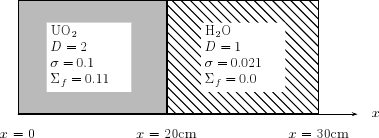
\psfig{file=images/img1.png, width=254px}
       \caption[Esquema simple del reactor]{Modelo de un ractor nuclear unidimensional.
         Diagrama adaptado de \citet{diaz10}.}
     \label{fig:esquema}
  \end{center}
\end{figure*}

Como se puede apreciar, los parámetros que se mantienen constantes dentro de cada compartimiento, pueden verse
como una función constante por tramos que varía según $x$. Tenemos entonces:

\begin{eqnarray}
	D(x)=\left\{
		\begin{matrix}
			2 &\mbox{ si }& 0 < x < 20\\
			1 & \mbox{ si }& 20 < x < 30\\
		\end{matrix} \right.
\end{eqnarray}
\begin{eqnarray}
	\sigma(x)=\left\{
		\begin{matrix}
			0.1 &\mbox{ si }& 0 < x < 20\\
			0.021 & \mbox{ si }& 20 < x < 30\\
		\end{matrix} \right.
\end{eqnarray}
\begin{eqnarray}
	\Sigma_f(x)=\left\{
		\begin{matrix}
			0.11 &\mbox{ si }& 0 < x < 20\\
			0 & \mbox{ si }& 20 < x < 30\\
		\end{matrix} \right.
\end{eqnarray}

Por ende se puede reescribir la ecuación diferencial \ref{eq:ecuacionADiscretizar} de la siguiente manera:
\begin{eqnarray}
\label{eq:ecuacionADiscretizarParticular}
  -\dfrac{d}{dx}[D(x) \dfrac{d\phi}{dx}(x)] + \sigma(x) \phi(x)  &=& \lambda  \Sigma_f(x) \phi(x)
\end{eqnarray}
En este trabajo se halla una solución numérica para la ecuación diferencial anterior. El vector solución
representa la concentración de neutrones $\phi(x)$.

El resto de este trabajo se organiza de la siguiente manera: en la sección \ref{sec:discretizacion} se discretiza
el problema continuo mediante un algoritmo para el cómputo de la derivada y en la sección \ref{sec:computo} 
se utiliza este modelo discretizado para hallar una solución numérica para la concentración de neutrones
en estado estacionario del reactor nuclear. En la sección \ref{sec:conclusiones} se presentan las conclusiones
que se desprendieron de este trabajo.

\section{Discretización del problema}
\label{sec:discretizacion}
Vamos a discretizar el problema continuo que se presenta en la ecuación (\ref{eq:ecuacionADiscretizar}) 
utilizando un esquema centrado de orden dos. Para lograr esto se utilizará el algoritmo (\ref{eq:algoritmoDeDiscretizacion}),
\begin{eqnarray}
\label{eq:algoritmoDeDiscretizacion}
	f'(x) = \frac{f(x+h) - f(x-h)}{2h} - \frac{1}{12} f'''(\xi) h^2
\end{eqnarray}
donde $\xi \in int\{x-h,x+h\}$ y $h$ es el tamaño de un intervalo, el parámetro computacional.
Ahora entonces procedemos a discretizar el problema. Lo resolveremos por partes para simplificar los cálculos. Primero buscamos una aproximación para la expresión \ref{eq:discretizacionDelaDerivada}.
\begin{eqnarray}
\label{eq:discretizacionDelaDerivada}
	\dfrac{d}{dx}\bigg[D \dfrac{d\phi}{dx}(x)\bigg]  
\end{eqnarray}
Como ya dijimos, el valor de $D$ depende del valor de $x$, y la denotaremos $D(x)$. La misma expresión \ref{eq:discretizacionDelaDerivada}, se puede escribir, entonces, de la siguiente forma:
\begin{eqnarray}
\label{eq:discretizacionDelaDerivadaMejorado}
	\dfrac{d}{dx}[D(x) \phi'(x)]
\end{eqnarray}
Si aplicamos el algoritmo \ref{eq:algoritmoDeDiscretizacion} en la ecuación \ref{eq:discretizacionDelaDerivadaMejorado}, se obtiene la siguiente expresión:
\begin{eqnarray}
\label{eq:desarrolloDeLaDiscretizacion}
	\dfrac{d}{dx}[D(x) \phi'(x)] &=& \dfrac{D_{i+\frac{1}{2}}\phi'\big(x_{i+\frac{1}{2}}\big)  -  D_{i-\frac{1}{2}}\phi'\big(x_{i-\frac{1}{2}}\big)}     {2h} 
\end{eqnarray}
Donde hemos considerado:

\begin{eqnarray}
	x_i &=&x_0 + h*i \\
	\phi_i &\cong&\phi(x_0 + h.i)
\end{eqnarray}

De la misma manera, si aplicamos el algoritmo \ref{eq:algoritmoDeDiscretizacion} sobre los valores $\phi'(x_{i+\frac{1}{2}})$ y $\phi'(x_{i-\frac{1}{2}})$ en la ecuación \ref{eq:desarrolloDeLaDiscretizacion}, obtenemos el siguiente resultado:
\begin{eqnarray}
\label{eq:desarrolloDeLaDiscretizacion2}
	\dfrac{1}{2h} \bigg[	D_{i+\frac{1}{2}}.\bigg(\dfrac{\phi_{i+1} - \phi_{i}}{2h}\bigg) 	-
			D_{i-\frac{1}{2}}.\bigg(\dfrac{\phi_{i} - \phi_{i-1}}{2h}\bigg) \bigg]\\
\end{eqnarray}
Que se puede reordenar como:
\begin{eqnarray}
\label{eq:reemplazoDeLaDerivada}
	\dfrac{D_{i+\frac{1}{2}}(\phi_{i+1} - \phi_{i}) - D_{i-\frac{1}{2}}(\phi_{i} - \phi_{i-1})}{4h^2}
\end{eqnarray}
Si escribimos de nuevo la ecuación, pero ahora teniendo en cuenta la discretización recién realizada logramos la siguiente expresión:
\begin{eqnarray}
\label{eq:discretizacionNoFinal}
	-\bigg[\dfrac{D_{i+\frac{1}{2}}(\phi_{i+1} - \phi_{i}) - D_{i-\frac{1}{2}}(\phi_{i} - \phi_{i-1})}{4h^2}\bigg]
	+ \sigma_i \phi_i &=& \lambda \Sigma_{fi} \phi_i
\end{eqnarray}

Si realizamos cuentas sobre la ecuación \ref{eq:discretizacionNoFinal}, obtenemos la forma final discretizada:
\begin{eqnarray}
	-D_{i+\frac{1}{2}}.\phi_{i+1} + \\
	+(D_{i+\frac{1}{2}} + D_{i-\frac{1}{2}} + 4h^2.\sigma_i)\phi_{i} - \\
	-D_{i-\frac{1}{2}}\phi_{i-1} &=& \lambda 4h^2 \Sigma_{fi} \phi_i
\end{eqnarray}
Las condiciones de borde dadas son $\phi'(0) = 0$ y $\phi(30) = 0$. Asimismo, hay que tener en cuenta que para el caso $i = 0$ podemos aproximar la derivada como:
\begin{eqnarray}
	\phi'(0) &\cong & \dfrac{\phi_1 - \phi_0}{2h}
\end{eqnarray} \\
De lo que se deduce que
\begin{eqnarray}
	\phi_0 &=& \phi_1
\end{eqnarray}
Entonces, utilizando un esquema centrado de orden 2, se logro discretizar el problema continuo que se presentó en la sección \ref{sec:introduccion}. La discretización obtenida es la siguiente:
\begin{eqnarray}
	-D_{i+\frac{1}{2}}.\phi_{i+1} + \\
	+(D_{i+\frac{1}{2}} + D_{i-\frac{1}{2}} + 4h^2.\sigma_i)\phi_{i} - \\
	-D_{i-\frac{1}{2}}\phi_{i-1} &=& \lambda 4h^2 \Sigma_{fi} \phi_i
\end{eqnarray}
, con $\phi_0 = \phi_1$ y $\phi(30) = 0$.




\section{Cómputo de la concentración de neutrones en estado estacionario}
\label{sec:computo}
Esto pasado a forma matricial:
\begin{eqnarray}
\label{eqn:matrizA}
	 \left( \begin{array}{ccccc}
		D_{i+\frac{1}{2}} + 4h^2\sigma_i & -D_{i+\frac{1}{2}}  					& 0 		& 0 & \dots \\
		-D_{i-\frac{1}{2}} 		& D_{i+\frac{1}{2}} + D_{i-\frac{1}{2}} + 4h^2\sigma_i 	& -D_{i+\frac{1}{2}} & 0 & \dots \\
		0 & -D_{i-\frac{1}{2}}& D_{i+\frac{1}{2}} + D_{i-\frac{1}{2}} + 4h^2\sigma_i & -D_{i+\frac{1}{2}}  & \dots\\
		\vdots &\vdots&\ddots&\ddots&\\
		\end{array} 
	\right)
\end{eqnarray}
Llamemos A a la matriz (\ref{eqn:matrizA}), entonces lo que obtenemos es la ecuación \ref{eq:ecuacionDelAutovalor}
\begin{eqnarray}
\label{eq:ecuacionDelAutovalor}
A . \phi = \lambda . \phi
\end{eqnarray}

\section{Conclusiones}
\label{sec:conclusiones}
\warn Acá poner conclusiones, OBLIGATORIAMENTE
%
% References
%
\bibliography{paper}

\end{document}

